\begin{figure}[ht]
\centering
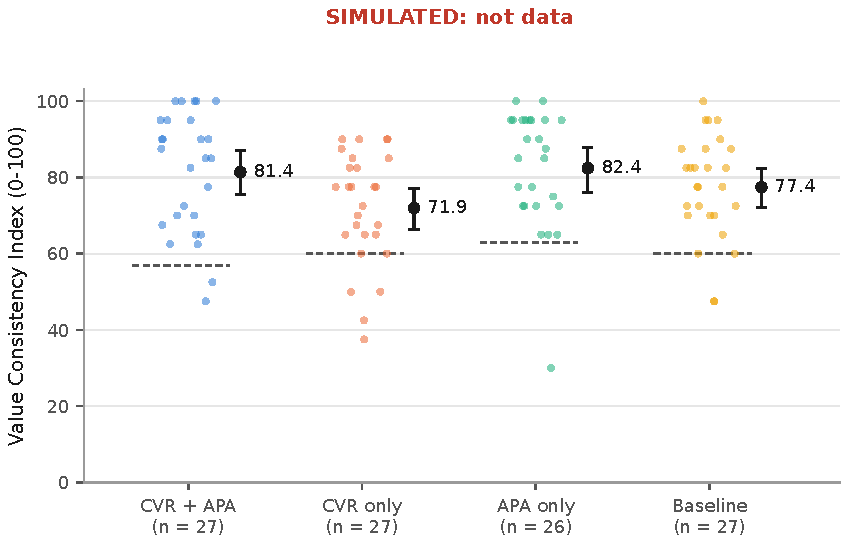
\includegraphics[width=\textwidth]{figures/fig_A1-A3_D3_vci_by_condition.pdf}
\caption{Value Consistency Index by Condition}
\label{fig:fig_A1-A3_D3_vci_by_condition}
\par\smallskip\begin{minipage}{\textwidth}\footnotesize\textit{Note.} SIMULATED: not data. Dots are participants. Black points with bars are condition means with 95\% bootstrap confidence intervals (4,000 resamples). Dashed lines mark the level a random chooser reaches in each condition (57, 60, 63 and 60), the reference of Hypothesis D3. Hypotheses A1-A3 compare CVR + APA with each other condition.\end{minipage}
\end{figure}

\begin{figure}[ht]
\centering
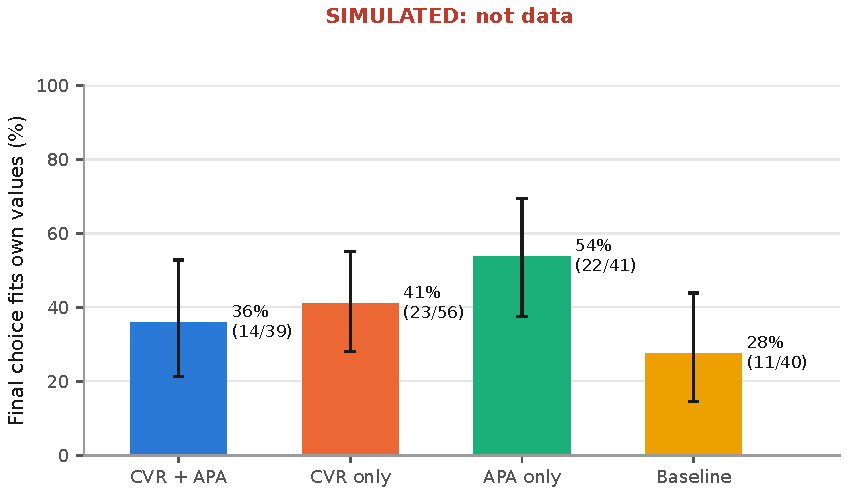
\includegraphics[width=\textwidth]{figures/fig_A4_final_fit_after_misfit_first_pick.pdf}
\caption{Final Choices That Fit the Participant's Values After a First Pick Against Them}
\label{fig:fig_A4_final_fit_after_misfit_first_pick}
\par\smallskip\begin{minipage}{\textwidth}\footnotesize\textit{Note.} SIMULATED: not data. Decisions in Scenarios 1-4 whose first pick was Misaligned or Strongly misaligned. Bars show the share whose final choice was Aligned or Weakly aligned, with exact (Clopper-Pearson) 95\% confidence intervals; counts are decisions. Hypothesis A4 compares the three conditions with a help step with Baseline.\end{minipage}
\end{figure}

\begin{figure}[ht]
\centering
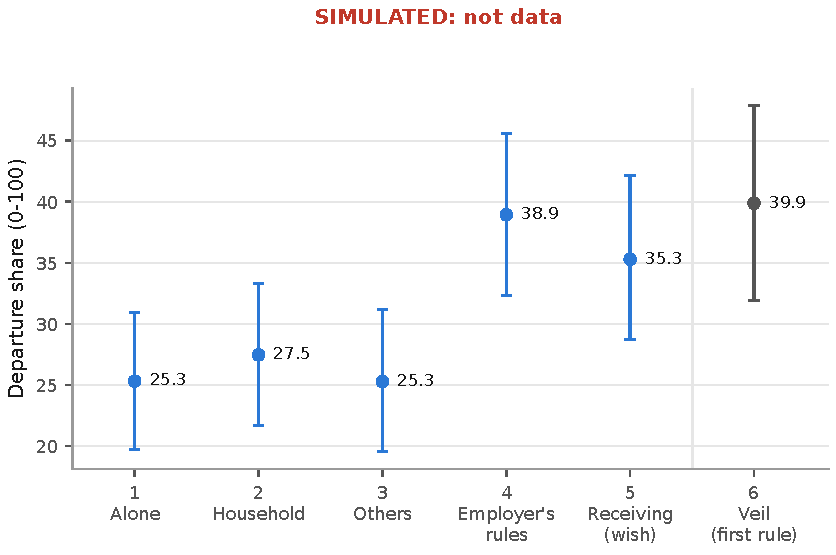
\includegraphics[width=\textwidth]{figures/fig_B1-B5_departure_by_scenario.pdf}
\caption{Departure From the Participant's Own Values in Each Scenario}
\label{fig:fig_B1-B5_departure_by_scenario}
\par\smallskip\begin{minipage}{\textwidth}\footnotesize\textit{Note.} SIMULATED: not data. Means with 95\% bootstrap confidence intervals. Departure share: 0 = the option closest to the values brought into the scenarios, 100 = the farthest. Scenario 6 uses the rule chosen before the prediction was shown (Hypothesis B5). The scenarios came in one fixed order.\end{minipage}
\end{figure}

\begin{figure}[ht]
\centering
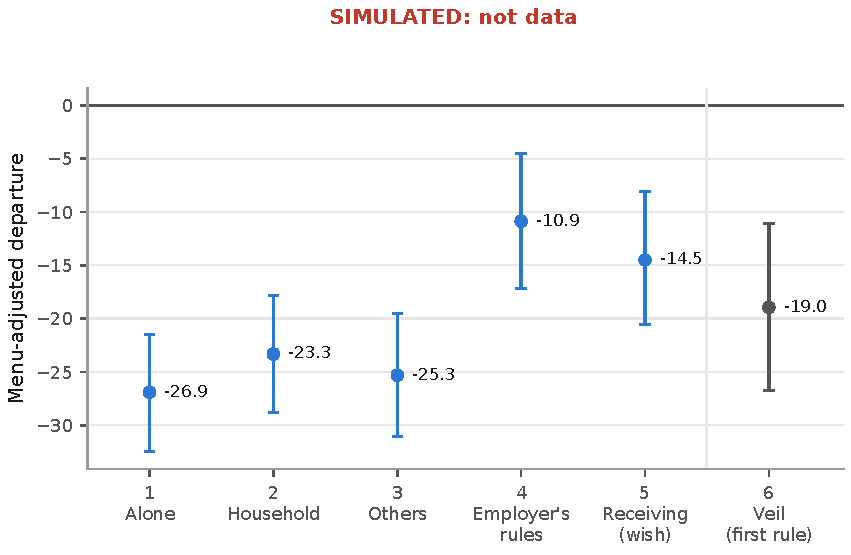
\includegraphics[width=\textwidth]{figures/fig_B1-B5_departure_by_scenario_menu_adjusted.pdf}
\caption{Departure From the Participant's Own Values in Each Scenario (Menu-Adjusted)}
\label{fig:fig_B1-B5_departure_by_scenario_menu_adjusted}
\par\smallskip\begin{minipage}{\textwidth}\footnotesize\textit{Note.} SIMULATED: not data. Means with 95\% bootstrap confidence intervals. Departure share: 0 = the option closest to the values brought into the scenarios, 100 = the farthest; the menu-adjusted value subtracts the mean departure share of all options on that menu. Scenario 6 uses the rule chosen before the prediction was shown (Hypothesis B5). The scenarios came in one fixed order.\end{minipage}
\end{figure}

\begin{figure}[ht]
\centering
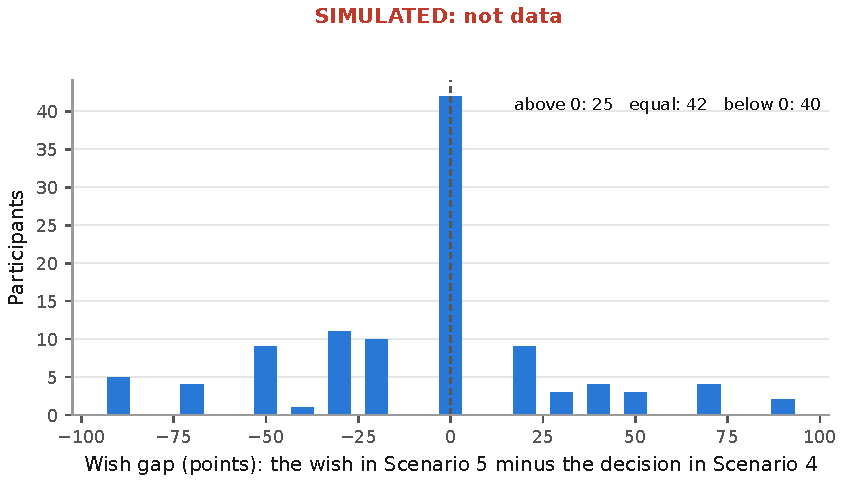
\includegraphics[width=\textwidth]{figures/fig_B6_wish_gap.pdf}
\caption{The Wish on the Receiving End Compared With the Participant's Own Decision}
\label{fig:fig_B6_wish_gap}
\par\smallskip\begin{minipage}{\textwidth}\footnotesize\textit{Note.} SIMULATED: not data. Both choices are judged on the values the participant held when Scenario 4 opened. Positive values: the wish fits the participant's values better than the decision (Hypothesis B6).\end{minipage}
\end{figure}

\begin{figure}[ht]
\centering
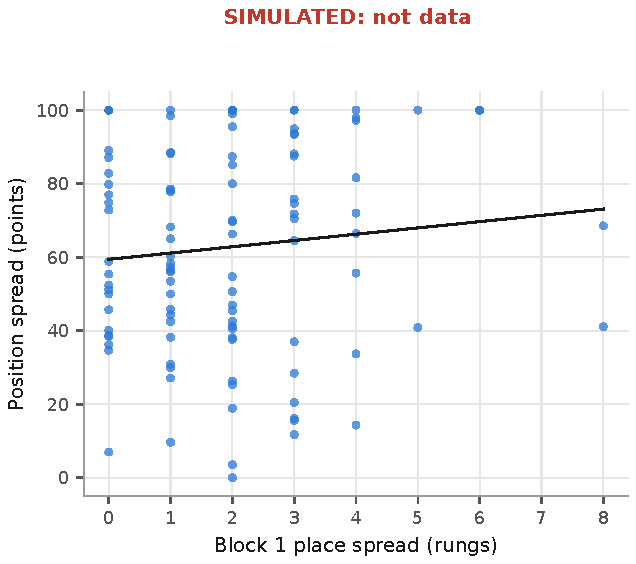
\includegraphics[width=\textwidth]{figures/fig_B7_place_spread_vs_position_spread.pdf}
\caption{Two Kinds of Spread}
\label{fig:fig_B7_place_spread_vs_position_spread}
\par\smallskip\begin{minipage}{\textwidth}\footnotesize\textit{Note.} SIMULATED: not data. Each dot is one participant; the line is a least-squares fit for orientation only (Hypothesis B7 uses rank correlations).\end{minipage}
\end{figure}

\begin{figure}[ht]
\centering
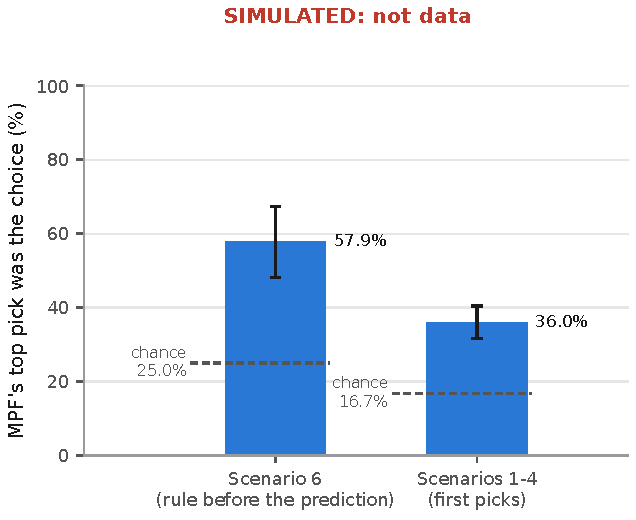
\includegraphics[width=\textwidth]{figures/fig_C1-C2_prediction_hit_rates.pdf}
\caption{How Often the Moral Prediction Function Named the Participant's Choice}
\label{fig:fig_C1-C2_prediction_hit_rates}
\par\smallskip\begin{minipage}{\textwidth}\footnotesize\textit{Note.} SIMULATED: not data. Bars: hit rates; intervals: exact 95\% (Scenario 6, Hypothesis C1) and 95\% bootstrap over participants (Scenarios 1-4, Hypothesis C2). Dashed lines: chance (one in four rules; one in six options).\end{minipage}
\end{figure}

\begin{figure}[ht]
\centering
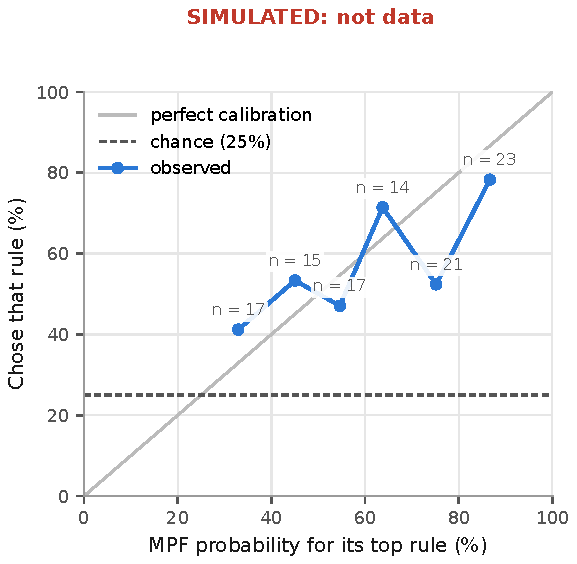
\includegraphics[width=\textwidth]{figures/fig_C3_calibration.pdf}
\caption{Calibration of the Prediction in Scenario 6}
\label{fig:fig_C3_calibration}
\par\smallskip\begin{minipage}{\textwidth}\footnotesize\textit{Note.} SIMULATED: not data. Participants grouped by the probability the Moral Prediction Function gave its top rule; the observed share who chose that rule (before seeing the prediction) in each group (Hypothesis C3).\end{minipage}
\end{figure}

\begin{figure}[ht]
\centering
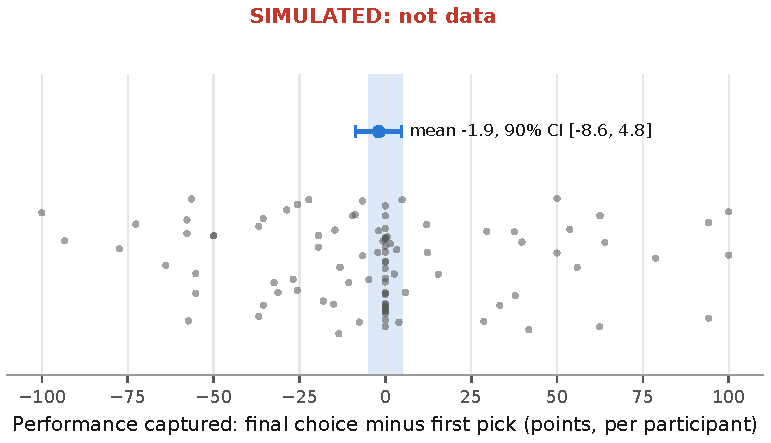
\includegraphics[width=\textwidth]{figures/fig_D1_performance_difference.pdf}
\caption{Performance of the Final Choice Compared With the First Pick}
\label{fig:fig_D1_performance_difference}
\par\smallskip\begin{minipage}{\textwidth}\footnotesize\textit{Note.} SIMULATED: not data. Each dot is one participant's mean difference over their decisions whose first pick went against their values and was followed by the condition's page. The shaded band is the preregistered equivalence margin; the interval is the 90\% confidence interval of the two one-sided tests (Hypothesis D1).\end{minipage}
\end{figure}

\begin{figure}[ht]
\centering
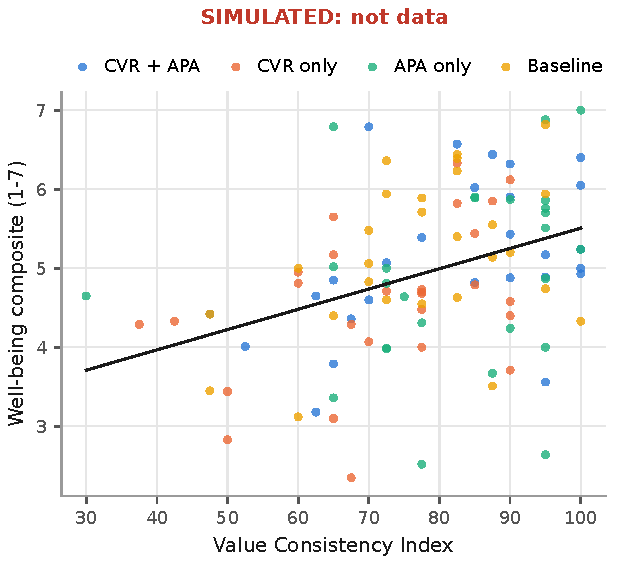
\includegraphics[width=\textwidth]{figures/fig_D4_vci_vs_wellbeing.pdf}
\caption{Value Consistency and Well-Being}
\label{fig:fig_D4_vci_vs_wellbeing}
\par\smallskip\begin{minipage}{\textwidth}\footnotesize\textit{Note.} SIMULATED: not data. Each dot is one participant; the line is a least-squares fit for orientation only (Hypothesis D4 adjusts for Stability, performance, age, gender, active minutes and condition).\end{minipage}
\end{figure}

\begin{figure}[ht]
\centering
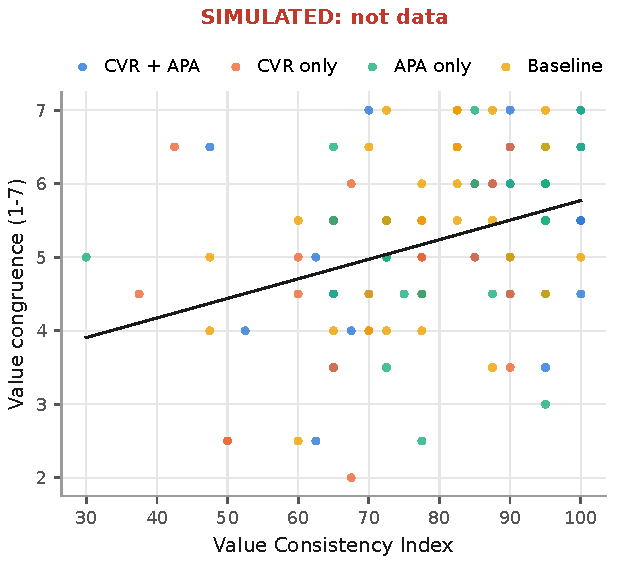
\includegraphics[width=\textwidth]{figures/fig_D5_vci_vs_value_congruence.pdf}
\caption{Value Consistency and Self-Reported Value Congruence}
\label{fig:fig_D5_vci_vs_value_congruence}
\par\smallskip\begin{minipage}{\textwidth}\footnotesize\textit{Note.} SIMULATED: not data. Each dot is one participant; the line is a least-squares fit for orientation only (Hypothesis D5 uses Spearman's rank correlation).\end{minipage}
\end{figure}
